\announcesection{Data Processing}

% Tracks
\displayonelarge{Tracking}{
    {\footnotesize
        2T solenoid magnet bends charged particles traversing trackers.
        Helical trajectory is used to calculated particle momentum/mass/charge.
    }
}{processing/IDbriefing_figure1}

% Jets
\displayonelarge{Jets}{
    {\footnotesize
        Determines energy of particles by seeing how many plates of metal they can go through.
        E-Cal for electrons/photons,
            H-Cal for hadronic particles.

    }
}{reconstruction/ATLAS_Detector_Schematic_black_particles}

% Flavor Tagging
\displayone{Flavor Tagging}{
    Uses a recurrent Deep Learning neural net (DL1r) to distinguish b-jets from light-jets.
    Primarily takes advantage of secondary vertexing and impact parameter jet properties
}{reconstruction/dl1_performance_ljet}

% Selection
\frame{
    \frametitle{Event Selection}
    \begin{columns} \begin{column}{0.5\textwidth}
        \begin{itemize}
            \item At least six jets total
            \begin{itemize}
                \item Central Jets: $|\eta| < 2.5$, $p_T > 40$ GeV
                \item Forward Jets: $2.5 < |\eta| \leq 4.5$, $p_T > 30$ GeV
            \end{itemize}
            \item Two \textit{anti}-b-tagged jets
            \begin{itemize}
                \item $ |\Delta \eta_{jj}| > 3.0 $,
                \item $M_{jj} > 1000$ GeV, and
                \item $p_{T,jj} < 65 $ GeV
            \end{itemize}
            \item At least 4 central, b-tagged jets
            \begin{itemize}
                \item $p_T > 40$ GeV
                \item paired up as reconstructed HH
                \item $ |\Delta \eta_{HH}| < 1.5 $
            \end{itemize}
            \item Using b-jet trigger DL1r 77\% working point,
                light jet acceptance of 0.59\%
        \end{itemize}
    \end{column} \begin{column}{0.5\textwidth}
        \begin{figure}
            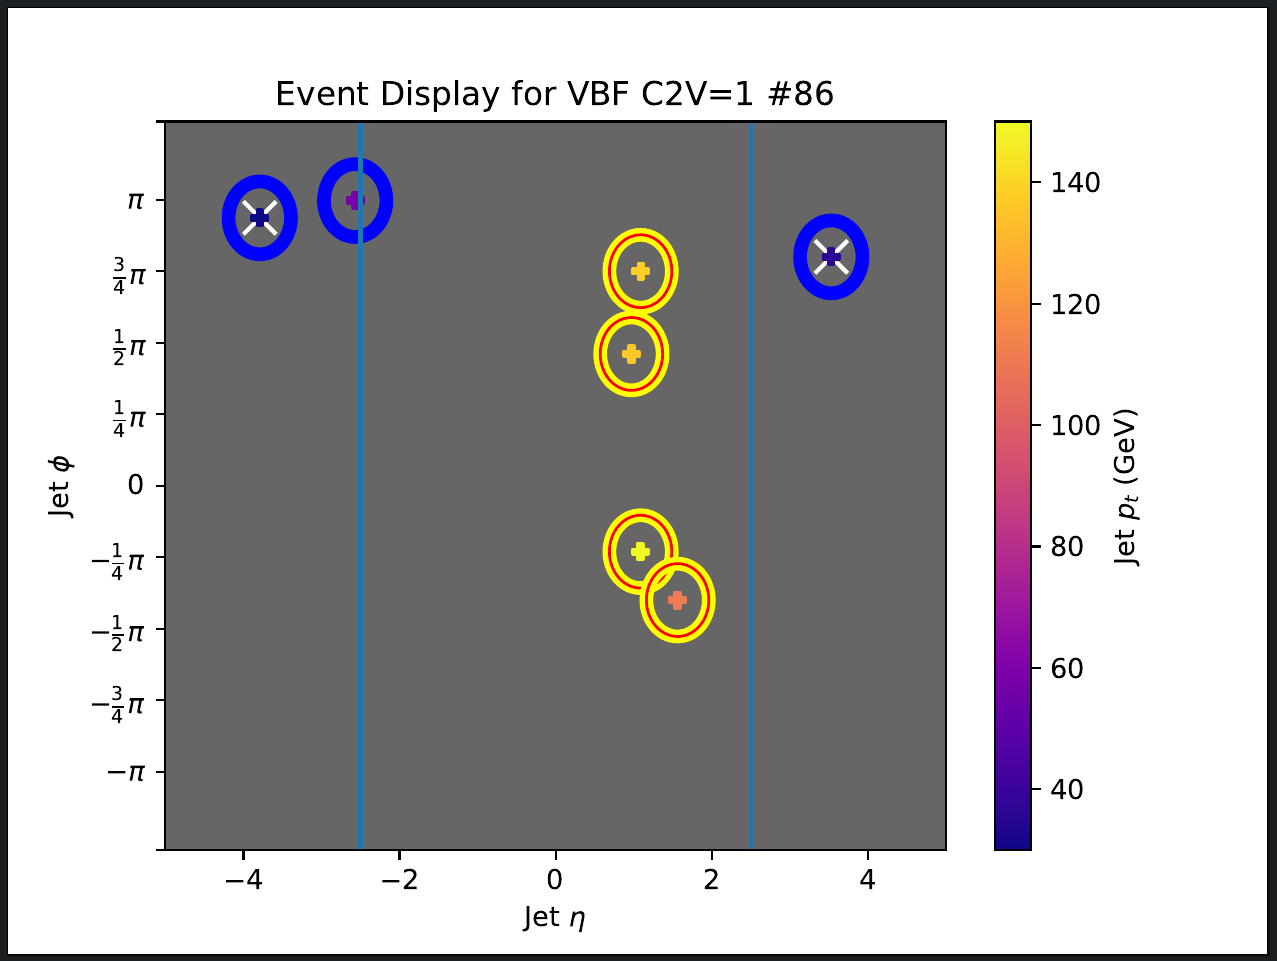
\includegraphics[width=\linewidth,height=0.9\textheight,keepaspectratio]{selection/event_display}
            \caption{\tiny Rings indicate jets;
                Yellow ring => b-tagged;
                Blue ring w/ white cross => VBF initial-scatter jets;
                ``+'' in center of rings => $p_T$;
                vertical lines denote "forward" vs "central" region.}
        \end{figure}
    \end{column} \end{columns}
}

% Background Events
\displayonelarge{Background Reweighting}{
    Posit that 2b-tagged events are kinematically similar to 4b-tagged background.
    Use NN ensemble to adjust kinematic differences, trained on ``control'' region of data.
}{selection/massplane_sig_all_4b_vbf_Xwt_1p5_k2V_0}

\displaytwo{Reweighting Performance}{}
{background/crypto-mean-stdBS-m-hh-Control-Region-1-no-rw-all-4binclusive}
{background/crypto-mean-stdBS-m-hh-Control-Region-1-NN-all-4binclusive}

%{background/crypto-mean-stdBS-X-wt-tag-Control-Region-1-no-rw-all-4binclusive}
%{background/crypto-mean-stdBS-X-wt-tag-Control-Region-1-NN-all-4binclusive}
%{background/crypto-mean-stdBS-dEta-hh-Control-Region-1-no-rw-all-4binclusive}
%{background/crypto-mean-stdBS-dEta-hh-Control-Region-1-NN-all-4binclusive}
